\documentclass[10pt, letter]{article}
\newcommand{\doctitle}{%
CS 4649/7649: RIP - Robot Intelligence - Planning}
\newcommand{\bigO}{\ensuremath{\mathcal{O}}}
\usepackage{graphicx}
\usepackage{float}
\usepackage{comment}
\usepackage{fancyvrb}
\usepackage{booktabs}
\usepackage[usenames,dvipsnames]{color}
\usepackage[center]{caption}
\usepackage{algorithm}
\usepackage[T1]{fontenc}
\usepackage[noend]{algpseudocode}
\usepackage{algorithm}
\usepackage[margin=1in]{geometry}
\usepackage[usenames,dvipsnames]{color}
\usepackage{hyperref}
\usepackage{xcolor}
\usepackage{amsmath}
\usepackage{subcaption}
\hypersetup{
  colorlinks,
  citecolor=Violet,
  linkcolor=Black,
  urlcolor=Blue}
%------------------------Included every possible package we might need ------------------------%
\begin{document}
\title{\textbf{\doctitle} \\\textsc{Project 1: Classical Sokoban Planner}}
  \author {Arvind Krishnaa Jagannathan, Zheng Yong, Luis Gustavo Souza Silva, Zhengyi Hu}%Others please check your names here
   \date{}
\maketitle

\section{Administrative}
\begin{itemize}
	\item This is a comprehensive report, with some plans incorporated into it. The plans are also available separately in the ``\textit{src/resources}`` directory.
	\item We have a \textit{README} file, which lists the directory structure of the attached \textit{zip} file. It also has the instructions for running the program.
	\item We also have outlined the participation of each of the members in the README file. Here is a brief summary of them.
		\begin{enumerate}
			\item \textbf{Luis}: PDDL definitions for Sokoban Part I for both the domain and each problem scenario. Also ensured that the planners work correctly on Windows.
			\item \textbf{Zheng}: Implemented the planning algorithm for Sokoban Part II, focusing on Branch optimization.
			\item \textbf{Zhengyi}: Implemented the planning algorithm for Sokoban Part II, focusing on state space compression and caching states into a hash map.
			\item \textbf{Arvind}: PDDL definitions for 3, 6, 10 disk Towers of Hanoi. Representation of domain and some minor fix-up to Sokoban Part II algorithm.
		\end{enumerate}
	Each of us have constructed the corresponding parts of this report. We have all read and reviewed each other's contribution to the report as well as the code.
\end{itemize}

\section{Pre-Project: Towers of Hanoi}
%Assigned to Arvind%
\subsection*{Planners Used}
The two classical planners which we are using for the Towers of Hanoi problem are the Blackbox planner \cite{kautz1998blackbox} (downloaded from \url{http://www.cs.rochester.edu/~kautz/satplan/blackbox/blackbox-download.html}) and the FF planner \cite{hoffmann2001fast} (downloaded from \url{http://fai.cs.uni-saarland.de/hoffmann/ff/FF-v2.3.tgz}). The definition of the Towers of Hanoi domain, as well as the representation of the initial state of the problem (from Figure \ref{fig1}) are in the corresponding PDDL files, namely \textit{hanoi-domain.pddl} and \textit{hanoi-3.pddl}.

\begin{figure}[h!]
  \centering
    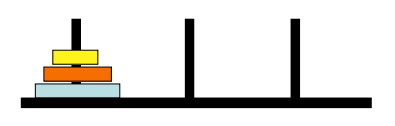
\includegraphics[scale = 0.3]{images/hanoi1}
    \caption{Towers of Hanoi with 3 disks}
  \label{fig1}
\end{figure}

\subsection{Questions}
\subsubsection*{1. Explain the method by which each of the two planners finds a solution}
\textbf{BlackBox}- The Blackbox planning algorithm essentially represents the PDDL representation of a problem as a set of Boolean satisfiability problems (SAT), which are then solved using a variety of SAT solvers (such as satz, walksat and chaff) to produce a plan.
In order to construct the SAT problem, Blackbox uses the \textsc{GraphPlan} algorithm to construct a plan graph for the given problem representation. This plan graph is then ``translated'' to the SAT problem representation. This is outlined briefly below:

The \textsc{GraphPlan} algorithm works by constructing a planning graph out of a \textsc{Strips} representation, which will propagate actions/operators across different ``layers'' along with their ``mutex'' pre-conditions. So at every stage there will be a list of actions, which have mutually exclusive pre-conditions. The plan generated by \textsc{GraphPlan} will be a sub-graph of the plan graph such that, all the conditions of the initial and final state are incorporated without there being any ``conflicting'' actions. As described by Kautz et. al \cite{kautz1996encoding}, each state in this solution graph can be encoded into propositional logic. This can be done by adding propositions of the form,
\begin{center}
$Precondition_i$ $\implies$ $Action_j$
\end{center}
At each layer of the solution sub-graph, clauses/fluents can be resolved away to result in a compact propositional logic representation of the plan graph. This list of proposition corresponds to the ``translation'' of the plan graph into a SAT problem. Then any available SAT solver can be applied on this problem which (although NP-complete in theory) with reasonable assumptions be completed in exponential time. ($O(n^3)$)

\textbf{FF Planner} - The fast-forward planning algorithm utilizes \textsc{GraphPlan} as an admissible (and informed) heuristic to solve the planning problem using a search algorithm across the set of permissible states in the state space. FF planner works as follows: it sets up a relaxed solvable sub-problem ($S\prime$) of the original problem ($S$).Then \textsc{GraphPlan} is applied on the relaxed sub-problem; the length of the solution plan sub-graph is then treated as a heuristic to guide the state space search algorithm for a plan to the original problem. This takes into account the positive interactions between various facts in the problem.

FF uses the enforced hill climbing algorithm to search for valid solutions. Using the length of the relaxed \textsc{GraphPlan} solution as a heuristic, the enforced hill climbing algorithm evaluates the direct successors of a search state S. Until a state ($S\prime$) is found with a better heuristic evaluation than $S$, the search goes one step further.

Thus in summary both \textit{\textbf{FF}} and \textit{\textbf{Blackbox}} algorithms use the \textsc{GraphPlan} algorithm, however \textit{Blackbox} uses it in a more direct way, to set up the SAT problem. In \textit{FF}, \textsc{GraphPlan} is used simply as a heuristic measure for the enforced hill climbing algorithm.
Both the planners generated the same plan, which is in Figure \ref{plan1}.

\begin{figure}[h!]
  \centering
    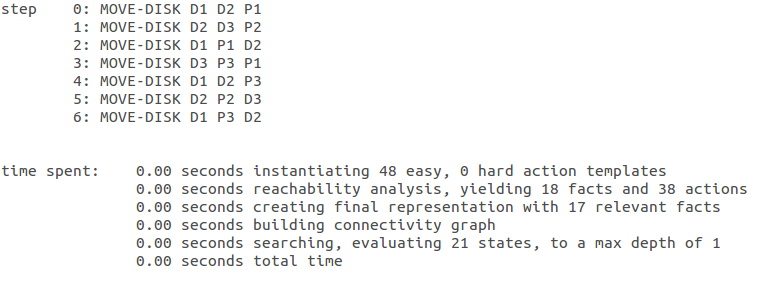
\includegraphics[scale = 0.5]{images/hanoi-3}
    \caption{Plan for Towers of Hanoi with 3 disks (generated from FF planner)}
  \label{plan1}
\end{figure}

\subsubsection*{2. Which planner was fastest?}
\label{subsubsec_2}
Both the algorithms were run on the same Linux box, and using the \textit{time} command the time taken for them to produce plans were measure. Clearly the \textbf{FF} algorithm was the fastest among the two, with the following time measures \\
\begin{itemize}
\item FF - 0.004s
\item Blackbox - 0.011s
\end{itemize}
This shows that \textbf{FF} is 2.75 times faster than \textbf{Blackbox}. This is pretty much expected from theory since the time complexity for each of the algorithms are,
\begin{center}
	O(\textit{Blackbox}) = O(\textsc{GraphPlan'}) + O(\textit{SAT Solver})\\
	O(\textit{FF}) = O(\textsc{GraphPlan}) + O(\textit{Enforced Hill Climbing})\\
	O(\textit{Enforced Hill Climbing}) = O(iterations x successors),\\
	O(\textit{SAT Solver}) = O($2^n$)
\end{center}
Clearly the SAT solver's exponential time complexity, as well as the time complexity of the complete \textsc{GraphPlan} algorithm for \textit{Blackbox} vs. that of the relaxed \textsc{GraphPlan} as well as that of \textit{Enforced Hill Climbing} for the \textit{FF} make it obviously slower than FF; this has been shown by using the towers of hanoi state and domain PDDL description multiple times (to get an average measure) with Blackbox and FF.
\subsubsection*{3. Explain why the winning planner might be more effective on this problem}
Its pretty obvious that the length of a plan in case of the Towers of Hanoi problem are a similar order of magnitude as that of the total number of states ($2^n - 1$ steps and $3^n$ states). In case of the \textbf{FF} planner, \textsc{GraphPlan} is used only as a heuristic and that too for a relaxed subset. \textit{FF}'s major component is the local-search algorithm, which means it does not have to necessarily traverse all the states in order to obtain a solution.

\textit{Blackbox} on the other needs to explicitly construct the mutex graph for every level until a solution is obtained. In case the state space is large (like 10 disks in the Towers of Hanoi problem), the construction of a complete plan graph is memory prohibitive and will not be effective on larger instances of this problem (it actually does not give plans for even 6 disks on my machine after 1 minute of execution). Another major issue with \textit{Blackbox} is that several levels of the \textsc{GraphPlan} algorithm may lead to the same set of SAT problems, which will remain unsatisfiable. \textit{Blackbox} is bound to be less effective in similar large state problems, since it seems to perform the same computation multiple times.

%-----------------------------------End of Problem 1 ---------------------------------------------%

\section{Project Part I: Sokoban PDDL}
%Assigned to Luis%

\begin{figure}[h]
  \centering
    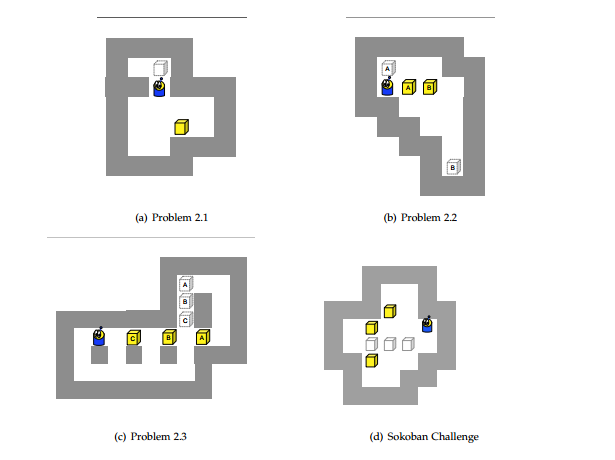
\includegraphics[scale = 0.5]{images/sokoban}
    \caption{Sokoban Problems}
  \label{fig2}
\end{figure}

\textbf{Note}: We have made the assumption that the \textit{planner can move any box to any target square}. This assumption is carried over to Part II as well.

The Sokoban's domain definition was created with the guideline idea of keeping it simple. Then, we followed the steps:

\begin{enumerate}
\item Identify the constants
\item Identify the fluents
\item Identify the actions
\end{enumerate} 

The first step is to identify the constants we evaluate possible elements that could be part of the domain. From this, constants like \textit{robot}, \textit{box} and \textit{location} appeared. However the problem only have one robot and is more natural to think about each box by its location instead of any kind of specific identification. Because of this, we moved on with only the \textit{location} constant.

The second step is to identify fluents related to this problem. We had a lot of possible fluents, most of them were related to the idea of using the constants already eliminated. However, to keep it simple, the fluents used were:

\begin{itemize}
\item \textbf{in(?loc)} - true if the robot is at location loc;
\item \textbf{boxAt(?loc)} - true if there is a box at location loc;
\item \textbf{isLeft(?loc ?loc)} - true if loc(1) is at left of loc(2);
\item \textbf{isRight(?loc ?loc)} - true if loc(1) is at right of loc(2);
\item \textbf{isUp(?loc ?loc)} - true if loc(1) is at up of loc(2);
\item \textbf{isDown(?loc ?loc)} - true if loc(1) is at down of loc(2).
\end{itemize} 

Finally, the last step is to identify the actions. For the Sokoban domain, the robot can move or push a box in the up, down, right and left directions, provided that there is no box on the way. After defining each action in respect to its preconditions, add list and delete list we could define the following:

\begin{itemize}
\item \textbf{MOVE-<UP,DOWN,RIGHT or LEFT>(?loc-to ?loc-from)};
\item \textbf{PUSH-<UP,DOWN,RIGHT or LEFT>(?box-loc ?loc ?loc-to)}.
\end{itemize} 

Done that, the next part of the question was to define each problem using this domain. For that, each grid position, from top to botton, and left to right, received a nickname of a alphabet letter. Then, all the constraints of linking these grid positions were defined using the fluent \textit{isUp}, \textit{isDown}, \textit{isRight}, \textit{isLeft} and the initial and goal state using the fluents \textit{in} and \textit{boxAt}.

\subsection{Questions}
\subsubsection*{1. Show successful plans from at least one planner on the three Sokoban problems in Figure \ref{fig2} (1-3). The challenge problem is optional}
Using the PDDL definitions for the domain, the FF planner was able to find solutions for all the problems and to the challenge. The result plan of each problem is shown on the Figures \ref{fig_prob2_1}, \ref{fig_prob2_2}, \ref{fig_prob2_3} and \ref{fig_prob2_challenge}.

\begin{figure}[h!]
  \centering
    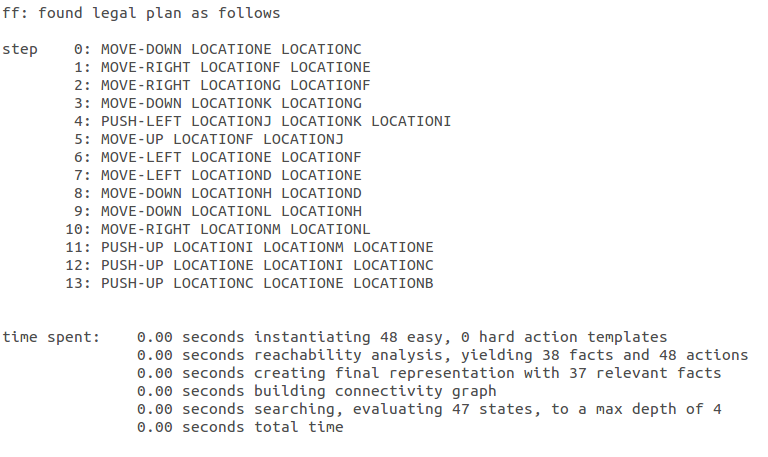
\includegraphics[scale = 0.4]{images/FF_Solution_p2_1}
    \caption{Sokoban Problem 2.1}
  \label{fig_prob2_1}
\end{figure}

\begin{figure}[h!]
  \centering
    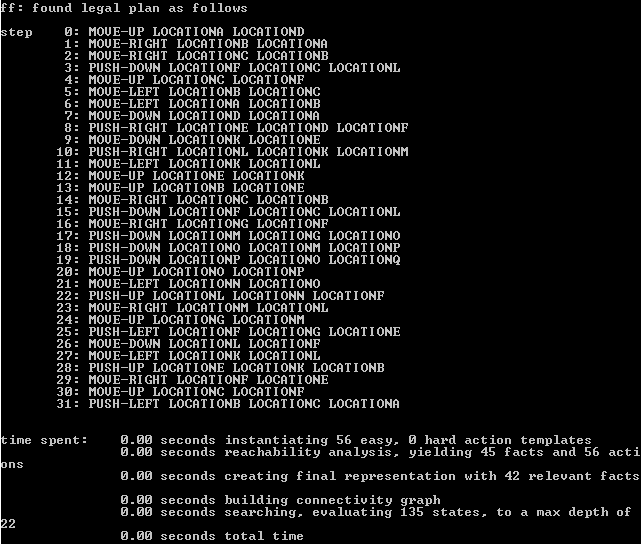
\includegraphics[scale = 0.4]{images/FF_Solution_p2_2}
    \caption{Sokoban Problem 2.2}
  \label{fig_prob2_2}
\end{figure}

\begin{figure} [h!]
\centering
\begin{subfigure}{.5\textwidth}
  \centering
  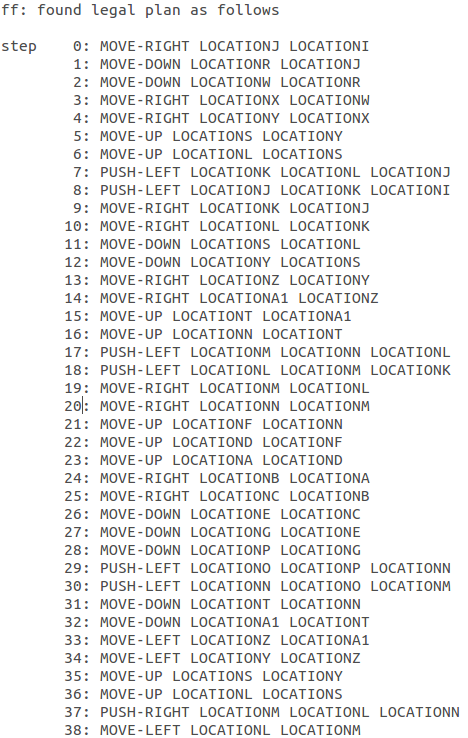
\includegraphics[scale = 0.3]{images/FF_Solution_p2_3_1}
\end{subfigure}%
\begin{subfigure}{.5\textwidth}
  \centering
  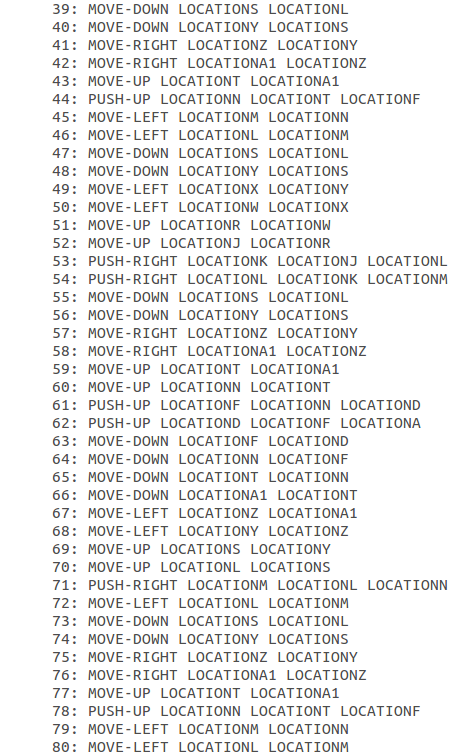
\includegraphics[scale = 0.3]{images/FF_Solution_p2_3_2}
\end{subfigure}\\
\begin{subfigure}{\textwidth}
  \centering
  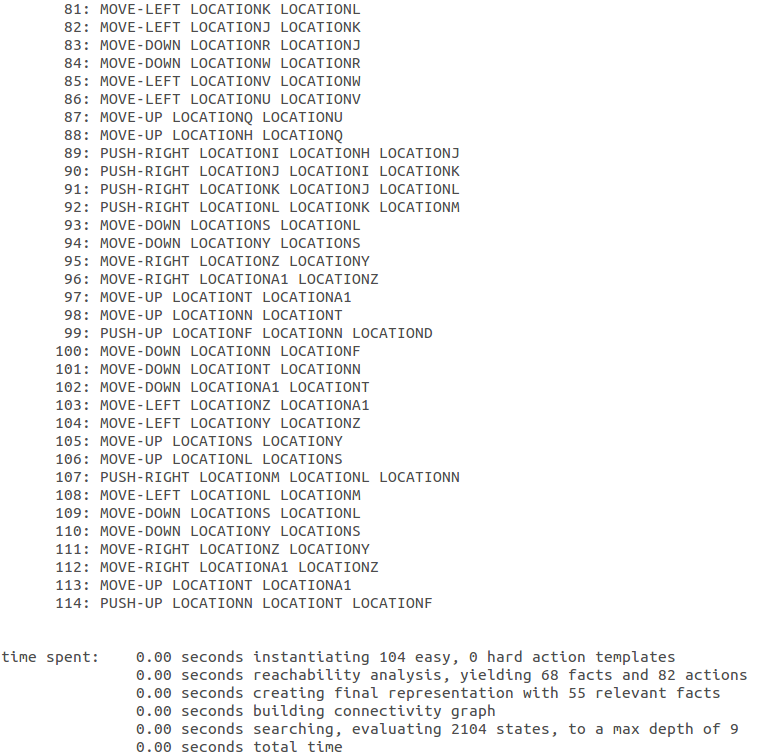
\includegraphics[scale = 0.3]{images/FF_Solution_p2_3_3}
\end{subfigure}%
\caption{Sokoban Problem 2.3}
\label{fig_prob2_3}
\end{figure}

\begin{figure} [h!]
\centering
\begin{subfigure}{.5\textwidth}
  \centering
  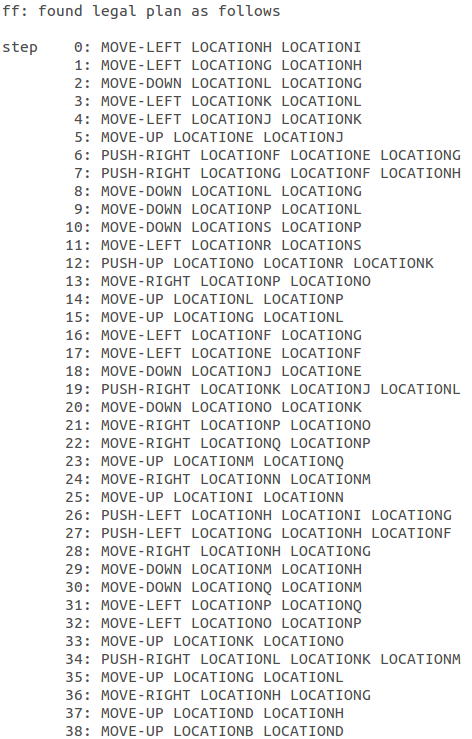
\includegraphics[scale = 0.3]{images/FF_Solution_p2_challenge_1}
\end{subfigure}%
\begin{subfigure}{.5\textwidth}
  \centering
  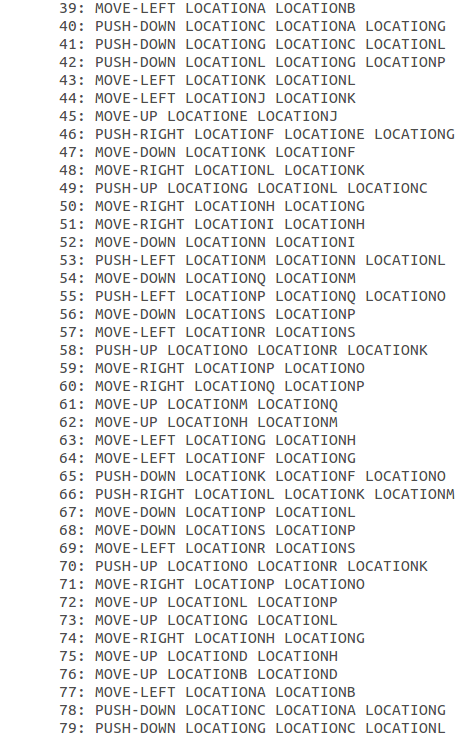
\includegraphics[scale = 0.3]{images/FF_Solution_p2_challenge_2}
\end{subfigure}\\
\begin{subfigure}{\textwidth}
  \centering
  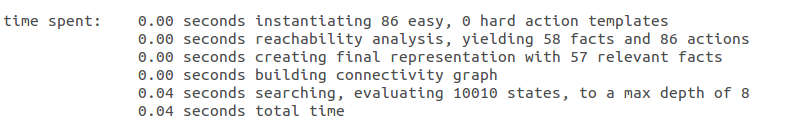
\includegraphics[scale = 0.3]{images/FF_Solution_p2_challenge_3}
\end{subfigure}%
\caption{Sokoban Challenge}
\label{fig_prob2_challenge}
\end{figure}

In order to make the solutions more readable and easier to verify, lets consider that when a robot moves for up, down, right or left direction it will be represented by a lowercase \textbf{u}, \textbf{d}, \textbf{r} or \textbf{l}, respectively. For the push actions of moving the box up, down, right or left, the capital letters \textbf{U}, \textbf{D}, \textbf{R} and \textbf{L} will be used. Thus, the solutions found can be represented as the strings shown below.

\begin{tabular}{ c l }
  &\\
  \textbf{Problem 2.1} & drrdLullddrUUU\\
  &\\
  \textbf{Problem 2.2} & urrDulldRdRluurDrDDDulUruLdlUru\\
  &\\
  \textbf{Problem 2.3} & rddrruuLLrrddrruuLLrruuurrdddLLddlluuRlddrruUllddlluu\\
                       & RRddrruuUUddddlluuRlddrruUllllddlluuRRRRddrruuuddd\\
                       & lluuRlddrruU\\
  &\\
  \textbf{Challenge}   & lldlluRRdddlUruulldRdrruruLLrddlluRuruulDDDlluRdrUrrd\\
                       & LdLdlUrruullDRddlUruuruulDD\\
\end{tabular}

\subsubsection*{2. Compare the performance of two planners on this domain. Which one works better? Does this
make sense, why?}

As an overview, the \textit{FF}'s planner performed better than \textit{Blackbox}. The \textit{FF}'s planner was able to find results for all problems, including challenge, in few seconds. On the other hand, the \textit{Blackbox} planner only managed to find the results from the first two problems and stopped on the others after using all the hardware resources. These results were expected since, as stated in Section \ref{subsubsec_2}, the \textit{FF}'s planner have a lower asymptotic complexity and use an heuristic function to choose the best option of what expand next. Thus, is more likely to have better time and space complexities than the \textit{Blackbox}.

\subsubsection*{3. Clearly PDDL was not intended for this sort of application. Discuss the challenges in expressing geometric constraints in semantic planning}

While solving this problem is possible to notice that are two approaches. The first one requires a previous knowledge of a solution, and the developer states that a specific box goes to a specific location. The second approach, there is no kind of identification for the boxes, and this is the one we used as a solution. Independently of the approach, the domain contains a grid on which the robot should move. Thus, it is necessary to come up with a way to express when the robot can, or cannot, move between two locations if there is a wall or a box in between. Also, is necessary to express when the robot is allowed to do something, like moving between two empty adjacent squares. Thus, all these logic expressions were used to represent geometric constraints like collisions between the robot and the walls or boxes.

Also, we had to clearly discretize the continuous space (into a set of boxes on a grid), which may then introduce resolution errors (not in this problem, but discretization may result in ``squares'' which are obstacles although in the continous domain there would have been space for navigation). 

\subsubsection*{4. In many cases, geometric and dynamic planning are insufficient to describe a domain. Give
an example of a problem that is best suited for semantic (classical) planning. Explain why a
semantic representation would be desirable}

The classical planners have a variety of best suited problems, like in logistics, manofacturing, and management. One example is the DART system used for military logistics. Logistics are better expressed by a set of logical expressions to specify complex operations not related to the kinect motion.

%------------------------------------End of Problem 2 -------------------------------------------------%

\section{Project Part II: Sokoban Planner}
%Assigned to James and Stango%
%Some by Arvind%
In this part of the project, we came up with our own representation of the Sokoban domain. The domain has the following specifications:
\begin{itemize}
	\item \textbf{Geometry/Grid}: A world represented as a $M$ x $N$ grid. The Sokoban domain's geometry is defined by $M$ rows and $N$ columns, where each ``cell'' in the map has the same dimensions as the box.
	\item \textbf{Walls}: A wall is any of the grey boundary of the world, as well as a logical extension of the wall to fit the map. For instance, looking at the first problem in Figure \ref{fig2}, the top most row is entirely made up of walls (although there is some white space in the top right, that cannot be logically reached by the man and hence is a ``wall''. In our representation a wall is defined by the constant $W$.
	\item \textbf{Boxes}: In the grid for each problem, we define a constant $B$ which corresponds to whether the box is present in that particular cell of the grid. We have assumed again that any box can be moved to any target square.
	\item \textbf{Target}: This is the target square where any box can be moved. Represented as $D$.
	\item \textbf{Man}: This represents the starting square in which the man is present. Represented in the grid as $M$.
	\item \textbf{Empty Squares}: These correspond to squares which are within the boundaries of the ``walls'' and can be occupied by a man or a box. Represented by $*$.
\end{itemize}

\begin{comment}
\textbf{Note}: In our plans, we do not explicitly show the man. Instead we show one or more boxes changing their position with respect to the previous step. Since the man will be in one of the adjacent spaces of the box (left, right, top or bottom) we have effectively treated the man and the box as one ``logical'' unit. This can be verified in the plans as well by tracing the location change of the various boxes.

In other words, we don't have actions such as \textsc{Push}, since we treat the box to be able to \textsc{Move} automatically based on the available white space. However we do respect the geometric constraints of the presence of the man (i.e., the box will not move to a location where a man should have been standing).
\end{comment}

\subsection*{Representation of the Domain}
Now that we have defined the components of the representation, we have defined the Sokoban domain for each of the 4 problems. Each problem has a ``\textit{input}'' map file which has the following header:
\begin{verbatim}
	{Rows} {Columns} {Number of boxes}
\end{verbatim}
Below the header is the grid based representation of the domain. The grid is a $Row$ x $Column$ matrix, where each element is a single character as defined previously. The 4 Sokoban problems (including the challenge problem) and their corresponding state representation as per our domain definition are presented in Figures \ref{soko1}, \ref{soko2}, \ref{soko3}, \ref{sokoC} respectively.

\begin{figure} [h!]
\centering
\begin{subfigure}{.5\textwidth}
  \centering
  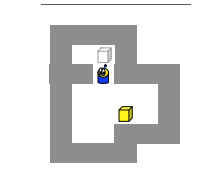
\includegraphics[scale = 0.5]{images/sokoban1}
\end{subfigure}%
\begin{subfigure}{.5\textwidth}
  \centering
  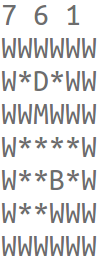
\includegraphics[scale = 0.5]{images/sokoban1-plan}
\end{subfigure}%
\caption{Sokoban Problem 2.1 and its corresponding representation}
\label{soko1}
\end{figure}

\begin{figure} [h!]
\centering
\begin{subfigure}{.5\textwidth}
  \centering
  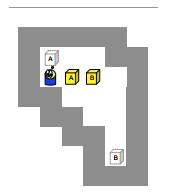
\includegraphics[scale = 0.5]{images/sokoban2}
\end{subfigure}%
\begin{subfigure}{.5\textwidth}
  \centering
  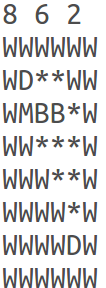
\includegraphics[scale = 0.5]{images/sokoban2-plan}
\end{subfigure}%
\caption{Sokoban Problem 2.2 and its corresponding representation}
\label{soko2}
\end{figure}

\begin{figure} [h!]
\centering
\begin{subfigure}{.5\textwidth}
  \centering
  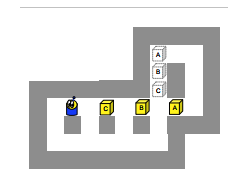
\includegraphics[scale = 0.5]{images/sokoban3}
\end{subfigure}%
\begin{subfigure}{.5\textwidth}
  \centering
  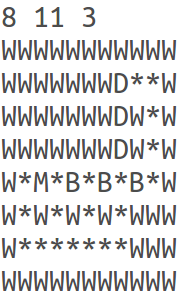
\includegraphics[scale = 0.5]{images/sokoban3-plan}
\end{subfigure}%
\caption{Sokoban Problem 2.3 and its corresponding representation}
\label{soko3}
\end{figure}

\begin{figure} [h!]
\centering
\begin{subfigure}{.5\textwidth}
  \centering
  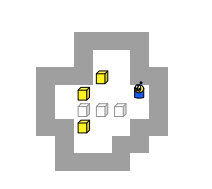
\includegraphics[scale = 0.5]{images/sokobanC}
\end{subfigure}%
\begin{subfigure}{.5\textwidth}
  \centering
  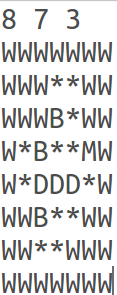
\includegraphics[scale = 0.5]{images/sokobanC-plan}
\end{subfigure}%
\caption{Sokoban Challenge and its corresponding representation}
\label{sokoC}
\end{figure}

\subsubsection*{Brief Outline of the Algorithm}
The algorithm is a simple implementation of the breadth-first search algorithm. The state is represented by the position of all the boxes and the position of the man (as per the representation). These arguments are integrated into a single \textit{long} integer. 

At the beginning of search, there is only one element in the search queue which is the initial state. Every time we look at a state, we first check if it is the final state (target configuration, where boxes ($B$) are in the places where target squares ($D$) are placed initially). If it is the final state, the program terminates with the solution. If not, we see if we can make any of the boxes move. If one of the boxes can be moved one step away in any direction, we take that move and add the new state into the queue. 

Also, every time we add a new state into the queue we check if the state is already explored (already in the queue). This is done by using a hash map. After adding all possible states that can be derived from the state we are dealing with right now, we move on to the next state in the queue. 

The program also terminates if the queue is empty, which indicates that there is no solution to the puzzle (and we report that).

\subsubsection*{Completeness, Speed and Efficiency}
We believe that our planner is complete as well as fast. We discuss more about this in the questions sections (Questions 3 and 4).
The state representation is pretty compact and really small in size. The processing on the input is also pretty fast since we cache the entire world state into a hash map. The maximum space complexity for the problem is $O(MXN)$ with $M$ rows and $N$ columns. However, this representation is pretty specific to the Sokoban domain. The only ``strong'' action in this domain is the \textsc{Push} action which we have incorporated into the state-space search. Our domain has nicely captured fluents such as \textsc{Location}, \textsc{Box-At} and so on within the grid representation.

\subsubsection*{Miscellaneous Pieces of Information}
We were able to capture most of the necessary pieces of information. We used a breadth-first search to explore the states, but we have not logged the explored states. So we are unable to report the number of states explored.
\begin{enumerate}
\item \textbf{Language Used}: C++
\item \textbf{Number of steps in plan}: We calculate the total number of steps it takes for every box to be moved to the target boxes. If there are $N$ steps, then our plan would correspond to $N$ world configurations, where the grid is represented as per the definitions stated above. There are currently some bugs in the printing logic, where in some steps, the man might make two or more movements as part of one step. After counting these mis-steps, our algorithm seems to take the same number of steps as FF. However, for transparency, we have the actual steps as reported by our algorithm below.
\begin{itemize}
\item Problem 1: \textbf{14} (FF was 14)
\item Problem 2: \textbf{29} (FF was 32)
\item Problem 3: \textbf{91} (FF was 115)
\item Challenge Problem: \textbf{48} (FF was 79)
\end{itemize}
\item \textbf{Computation Time}: We have compared our planner against FF (which was only able to produce the solution for all the 4 problems). Both planners were executed on the same system and the computation time is shown in Table \ref{tab1}.

\begin{table}[htbp]
\caption{Comparison of Computation Times}
\centering
\begin{tabular}{|r|r|r|}
\hline
\multicolumn{1}{|l|}{Problem} & \multicolumn{1}{l|}{FF Time (in s)} & \multicolumn{1}{l|}{Our Planner Time (in s)} \\ \hline
\multicolumn{1}{|l|}{} & \multicolumn{1}{l|}{} & \multicolumn{1}{l|}{} \\ \hline
1 & 0.005 & \textbf{0.004} \\ \hline

2 & 0.007 & \textbf{0.007} \\ \hline
3 & 0.021 & \textbf{0.019} \\ \hline
Sokoban Challenge & 0.043 & \textbf{0.025} \\ \hline
\end{tabular}
\label{tab1}
\end{table}
\textbf{Note}: Although it appears that our algorithm is ``faster'' than FF, that might not necessarily be the case, since our algorithm prints to a file, whereas FF prints to console. Due to the length of the plans, which need to be printed to the terminal, FF takes more time. FF has a self-reporting ``time spent'' parameter, and by using that as a comparison, we get the comparison as shown in Table \ref{tab2}.

\begin{table}[htbp]
\caption{Comparison of Computation Times (FF self-reported)}
\centering
\begin{tabular}{|r|r|r|}
\hline
\multicolumn{1}{|l|}{Problem} & \multicolumn{1}{l|}{FF Time (in s)} & \multicolumn{1}{l|}{Our Planner Time (in s)} \\ \hline
\multicolumn{1}{|l|}{} & \multicolumn{1}{l|}{} & \multicolumn{1}{l|}{} \\ \hline
1 & 0.00 & \textbf{0.004} \\ \hline

2 & 0.00 & \textbf{0.007} \\ \hline
3 & 0.00 & \textbf{0.019} \\ \hline
Sokoban Challenge & 0.04 & \textbf{0.025} \\ \hline
\end{tabular}
\label{tab2}
\end{table}

\item \textbf{Machine Vitals}: The input representation for each of the problems was very small (of the order of 50-60 bytes), and the output was also suitably compact. Our program can compile and run on any C++ compiler conforming to ANSI standard, and does not require too much of memory to run. The only memory constraints are the fact that we are loading the entire world onto a hash map, but again this is not very significant for the Sokoban domain as well as the BFS which explores every possible reachable state.

\item \textbf{States explored}: While performing the BFS, there were a number of states which were explored during the course of finding a valid plan. For each of the problems, the number of states explored are shown below:
\begin{itemize}
\item Problem 1: \textbf{14} (FF was 47)
\item Problem 2: \textbf{77} (FF was 135)
\item Problem 3: \textbf{344} (FF was 2104)
\item Challenge Problem: \textbf{954} (FF was 10010)
\end{itemize}
\end{enumerate}
\subsection{Questions}

\subsubsection*{1. Give successful plans from your planner on the Sokoban problems in Figure \ref{fig2} and any others}
We have a successful plan for the first Sokoban problem depicted in Figure \ref{sokoans1}. The format for the solutions of all the Sokoban problems are the same as in the Figure. But for lack of space, we do not include all the plans here. However, the plans for all the problems (1, 2, 3 and the challenge problem) can be found in the ``\textit{resources/Our\_Planner\_Solutions}'' directory.

Note that each step shows the world configuration with the position of the boxes, the man and ``empty space'' marked appropriately. We have an ``accomplished'' state, in which the boxes $B$ need to be present where the the target squares $D$ were present in the problem representation.
%-------------------Soko1------------------------
\begin{figure} [h!]
\centering
\begin{subfigure}{.3\textwidth}
  \centering
  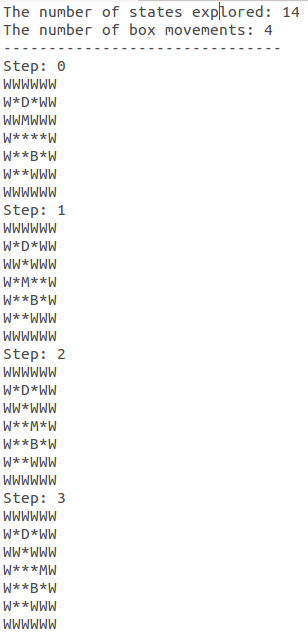
\includegraphics[scale = 0.35]{images/sokoban1-ans1}
\end{subfigure}%
\begin{subfigure}{.3\textwidth}
  \centering
  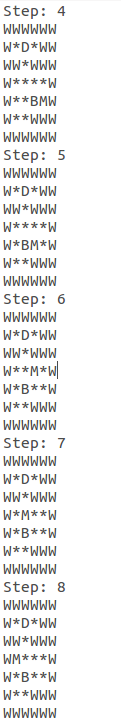
\includegraphics[scale = 0.35]{images/sokoban1-ans2}
\end{subfigure}%
\begin{subfigure}{.3\textwidth}
  \centering
  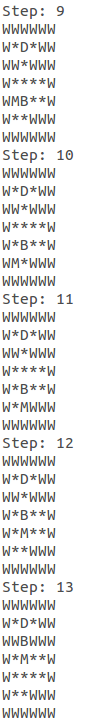
\includegraphics[scale = 0.35]{images/sokoban1-ans3}
\end{subfigure}\\
\begin{subfigure}{.5\textwidth}
  \centering
  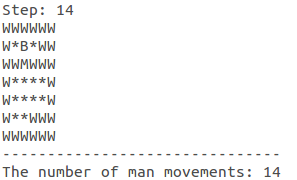
\includegraphics[scale = 0.35]{images/sokoban1-ans4}
\end{subfigure}%
\caption{Sokoban Problem 2.1's Plan}
\label{sokoans1}
\end{figure}
%-------------------Soko1------------------------

\subsubsection*{2. Compare the performance of your planner to the PDDL planners you used in the previous
problem. Which was faster? Why?}
As mentioned earlier, our planner was able to be almost as fast as the FF planner. Of course the time measure from Linux's \textit{time} utility may not be a fair comparison, since FF prints a ton of output to the console, which will take more time than printing to a file, which is what we are doing in our algorithm. Taking FF's internal time metric into account, most Sokoban problem gave a solution as 0.00s (Note that their level of precision is two digits, whereas \textit{time} has three digits of precision), except the last challenge problem, which FF reported to have taken 0.04s in total. However, we suspect FF might be not be as fast as our ``specialized'' Sokoban planner, since we have defined walls in the domain for this problem (as opposed to the case of FF where we did not). This definition enables our BFS to explore a lot less states than those explored by FF. 

Of course, we did not try to define a fluent called \textsc{Wall} along with its effects and pre-conditions in the PDDL definition for FF. Had we done that, FF might have possibly been faster, but that would have bloated the domain definition more that what it is right now!

\subsubsection*{3. Prove that your planner was complete. Your instructor has a math background: a proof ``is
a convincing argument.'' Make sure you address each aspect of completeness and why your
planner satisfies it. Pictures are always welcome.}
Basically our approach is Breadth First Search (BFS) with a little bit branch optimization, and it's easy to prove that it is complete.
The state is represented by several arguments: the position of every box and the position of the person.
And all these arguments are combined in one integer.
We use shift operations in C++ to set and get a specific argument (For example, the position of the person), which saves a lot of space.
Our algorithm searches for every possible move of the box, that is, as long as we can make a box move from the current state, we add this new state with the box moved to the new position. 
(And of course we assert that this new state is a state that we have not discovered yet. This is one of the branch optimizations)
We keep on doing this until we hit the final state or we run out of states.
If we hit the final state (with all boxes in designated positions), our algorithm ends and it prints out the plan we are looking for.
If the set of states is empty and we still don't find a solution, the algorithm also terminates with no solution.
Since BFS searches for every possible state that is reachable from the original state, if there exists a solution, we can always find it.
If there is no solution, since our algorithm only search for possible states, it will terminate with no solution.

Now there are two conditions for BFS to be complete \cite{cormen1996} and our definition of Sokoban domain satisfies both those conditions, namely
\begin{enumerate}
	\item Finite branching factor: The Sokoban world is clearly finite, and there can only be a finite number of possible states which we can explore with respect to any given state. Since the domain has a finite branching factor, the first condition is satisfied.
	\item Finite number of states: Clearly the Sokoban world has finite states. So there is no way for BFS to not converge to an answer if one exists (and will definitely report if one does not exist).
\end{enumerate}

Also our algorithm is optimal in terms of box moves (i.e., every step of moving the box to a square has the same cost). 
This is because every time we add a new state, it is a state that is one box-move away from the previous state.
Since we are using Breadth First Search, we can guarantee that our solution uses the least box moves.

\subsubsection*{4. What methods did you use to speed up the planning? Give a short description of each method
and explain why it did or didn't help on each relevant problem}
First of all we discard the new state that has already been explored.
This branch optimization cuts out a lot of useless branches, and it asserts that our algorithm terminates when there is no solution.
\\Also when checking if the state has been explored, we use hash map. 
Specifically, we use a large integer to represent the state, and throw the explored states into the hash.
So this saves the time needed for checking duplicate states.
\\Another branch optimization is that when we are in a state where one of the boxes has two adjacent sides facing the wall and this box is not in the designated position.
This box cannot be moved anyway because we need the man on one side of the box and we need the opposite side of the wall to be clear so that we can move. (In this case at least one side of these two is wall)
Therefore this state is itself a dead state. 
We will never make it to the final state in this case.

%---------------------------------End of Problem 3 ----------------------------------------------------%

\section{Post-Project: Towers of Hanoi Revisited}
%Assigned to Arvind%
Constructing a PDDL representation for the N-disk towers of hanoi is pretty simple by utilizing the following simple structures, for initializing the problem state
\begin{enumerate}
\item Each disk labeled $D_i$ is smaller than a disk labeled $D_{i+1}$. That is \texttt{(smaller $d_i$ $d_{i+1}$)}.
\item Every disk is smaller than each of the three poles (by definition).
\item The smallest disk (i.e., D1), and the two other poles (P1 and P2) are clear.
\item Every disk $D_i$ is \emph{on} the disk $D_{i+1}$. The largest disk D10, is \emph{on} the pole P3.
\item Every element $D_i$ is a disk
\end{enumerate}
The goal state is simply a conjunction (\textsc{And}-ing) of all the states mentioned in Step 4 above, except that the largest disk D10, is \emph{on} the pole P1.

The corresponding PDDL representations for the 6 disk and 10 disk towers of hanoi problem are present in the files ``hanoi-6.pddl'' and ``hanoi-10.pddl''.

Both \textbf{FF} and \textbf{Blackbox} planners were applied onto the PDDL representations, however only \textit{FF} was able to produce valid plans for the 6 disk and 10 disk problem. \textit{Blackbox} was unable to produce any results, due to relatively large nature of the state-space (I halted execution after 1 minute since the blackbox executable started running).

\subsection{Questions}
\subsubsection*{1. Give successful plans from at least one planner with 6 and 10 disks}
The plan for the towers of hanoi problem with 6 disks, generated by \textit{FF} is shown in Figure \ref{plan6}.

\begin{figure}[h!]
\centering
\begin{subfigure}{.5\textwidth}
  \centering
  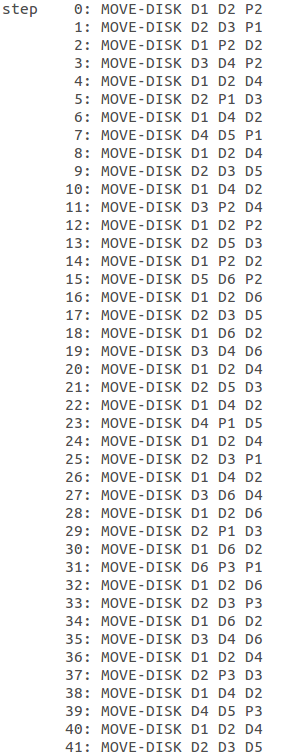
\includegraphics[scale = 0.3]{images/hanoi-6_1}
\end{subfigure}%
\begin{subfigure}{.5\textwidth}
  \centering
  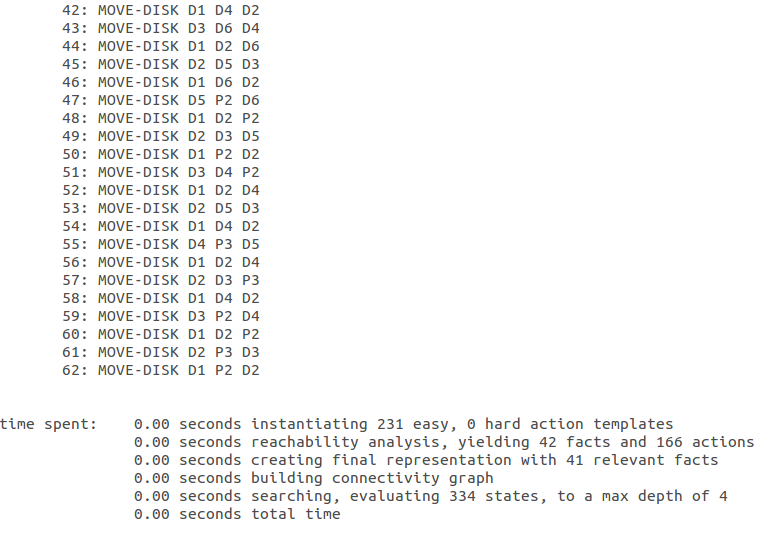
\includegraphics[scale = 0.3]{images/hanoi-6_2}
\end{subfigure}%
\caption{Plan for Towers of Hanoi with 6 disks}
\label{plan6}
\end{figure}

Clearly it has $2^6 - 1$ = 63 steps in the plan. Now the problem with 10 disks will have a plan of $2^{10} - 1$ = 1023 steps. The \textit{FF} planner produces a valid plan with 1023 steps, but for the lack of space it is not produced here. The plan is present under the ``resources/Hanoi Plans'' directory as ``hanoi-10-solutions''.

\subsubsection*{2. Do you notice anything about the structure of the plans? Can you use this to increase the
efficiency of planning for Towers of Hanoi? Explain}
One observation from the three plans generated (3, 6 and 10 disks) is that whenever there are odd number of initial disks, then the top most disk is moved onto the ``destination'' pole, and when there are even number of initial disks, then the top most disk is moved onto the ``middle'' pole.

Another noticeable aspect of the problem is that the towers of hanoi can be viewed as a simple recursive problem of moving the smaller $n-1$ disks from $P3$ to $P2$ then moving the largest disk from $P3$ to $P1$ followed by moving the $n-1$ disks from $P2$ to $P1$. This can be empirically verified - at every $(2^N - 1)^{th}$ step, if the initial number of disks $n$ are odd, then there will be $N-1$ disks on P2 and largest disk will be on P1. If the initial number of disks $n$ are even, then there will be $N-1$ disks on $P3$ and the largest will be on $P2$. Of course here, $0<N<=n$.

Thus the entire plan can be represented recursively (and efficiently) as: 
\begin{algorithm}
  \caption{Towers of Hanoi recursive definition}
  \begin{algorithmic}[1]
    \Function{Hanoi-Solver}{$N, P3, P2, P1$}
    \Comment{Move N disks from P3 to P1 (using P2 as intermediate)}
		\State \Call{Hanoi-Solver}{$N-1, P3, P1, P2$}
		\State \Call{Move}{$1, P3, P1$} \Comment{Move the largest disk from P3 to P1}
	  	\State \Call{Hanoi-Solver}{$N-1, P2, P3, P1$}
    \EndFunction
  \end{algorithmic}
\end{algorithm}

Thus this is a bottom-up approach in constructing a plan. All one needs to define are the ``macro'' propositions \textsc{Hanoi-Solver} and \textsc{Move} (which is applied when there is just the largest disk remaining on $P3$). The planner can then use this base condition (a.k.a ``macro'' proposition) and basically ``un-wind'' the call stack to generate sub-plans. The correct plan is then obtained by simply reversing the ``popped'' elements of the call stack.


\subsubsection*{3. In a paragraph or two, explain a general planning strategy that would take advantage of
problem structure. Make sure your strategy applies to problems other than Towers of Hanoi.
Would such a planner still be complete?}

A general recursive algorithm takes advantage of whenever there is a possibility of breaking down a problem into multiple smaller, but similarly structured problems, each if solved (and possibly in parallel if there is sufficient independence) can be ``combined'' to get the solution to the original problem. The generic recursive algorithm is:

\begin{algorithm}
  \caption{Recursive Planner}
  \begin{algorithmic}[1]
    \Function{Recursive-Planner}{$Prob_N$}
    \Comment{Solve a sub-problem}
    		\If{Some Terminal Condition}
			\State \Call{Terminal-Operation}{$Prob_1$} \Comment{Some constant terminal operation}
		\EndIf
		\State \Call{Recursive-Planner}{$Subset(Prob_N)$}
		\Comment{$Subset(Prob_N)$ might be $Prob_{N-1}$, $Prob_{\frac{N}{2}}$ etc,..}
    \EndFunction
  \end{algorithmic}
\end{algorithm}

There are a whole class of problems to which a recursive planner can be applied. For instance, this algorithm can be used in large scale map navigation problems, where loading an entire terrain in one go may be memory prohibitive.

There are two conditions for a planner to be complete,
\begin{enumerate}
\item \textbf{Produces a plan if there is one}: The recursive planner relies on all the sub-goals to complete their execution (or the recursion stack to be empty). So in case all the sub-goals reach their respective terminating condition, then all of them will reach completion (this is from an execution standpoint - different from the notion of completeness). If all the individual problems finish, then the top-level problem, which is basically a composition of these sub-problems will also produce a valid plan.

However, it is possible that even though the entire problem has a solution, one of the sub-problems may never reach completion -- this would cause the original problem to not produce a plan. Hence it cannot always be guaranteed that the planner produces a plan if there is a valid one.

\item \textbf{Reports that there is no plan if there is none}: The same sub-problem non-termination issue exists here as well. In case one of the sub-problems gets ``stuck'', there is no way for the original problem to terminate reporting that there is no plan. 
\end{enumerate}

However, if some sort of a terminating ``\textit{parameter}'' can be used to force the sub-problems to halt/report no solution, then we can guarantee completeness. In such a case the ``stack overflow'' issue will be resolved and both the conditions of completeness will be met. Basically, we need to ensure that the sub-problems will be forcibly terminated which will ensure that the main problem will always terminate as well! (Can almost be viewed as a ``stack unrolling'' limited algorithm, much like depth-limited search).

%----------------------------------End of Problem 4 ----------------------------------------------------%

\bibliographystyle{unsrt}
\bibliography{myrefs}
\end{document}
